\section{Experiments}


\subsection{Experimental Setups}
\paragraph{\textbf{Implementation.}}  For a comprehensive verification, we train our model on both open-source text-to-video models Wan2.1-14B-T2V \cite{wan2025wan} and Wan2.2-14B-T2V. We adopt a two-stage training process: in the first stage, we fine-tune for 2,000 steps on a 200K image-personalization dataset with a batch size of 96, updating only the patch embedding and self-attention modules to acquire basic personalization while preserving the base model’s capabilities. In the second stage, we finetune for 12,000 steps on a 750K video-personalization dataset with a batch size of 64, freezing the cross-attention modules to maintain text-following ability.  We use the Adam optimizer with a learning rate of $1e-5$ in the training process. The total training cost is approximately 30,000 GPU-hours. During training, the parameters of the reference branch in the Domain-MoT are initialized by copying those from the video branch, and the weight coefficient of the CCL Loss $\mathcal{L}_{\mathrm{C}}$ is set to $0.1$. During training, $K=4$, representing four domain attributes: real-world human, real-world object, background, and fantasy subject. Notably, domain attributes refer to the subject attributes in the generated video, rather than those in the reference images. Both the training and test sets use MLLM to annotate domain attributes. In addition, users can freely provide the corresponding domain attributes during their own inference.

%More details of the experiments are shown in Sec. B of the supplementary materials.

\begin{table*}[t]
\centering
\caption{\textbf{Quantitative results}. The best scores are shown in \textbf{bold}, and the second-best are \underline{underlined}. \textit{DomainShuttle} significantly outperforms the baselines in text controllability and most subject consistency metrics.}
\setlength{\tabcolsep}{6pt}
\resizebox{1.0\textwidth}{!}{
\begin{tabular}{lccccccccc}
\toprule
\multirow{2}{*}{Method} 
& \multicolumn{2}{c}{Video Quality} 
& \multicolumn{1}{c}{Text Controllability} 
& \multicolumn{4}{c}{Cross-Domain Subject Consistency} 
& \multicolumn{2}{c}{In-Domain Subject Consistency} \\
\cmidrule(lr){2-3} 
\cmidrule(lr){4-4} 
\cmidrule(lr){5-8} 
\cmidrule(lr){9-10}
& AES$\uparrow$ 
& MS$\uparrow$ 
& GMEScore$\uparrow$ 
& NANO-CLIP$\uparrow$ 
& Qwen-CLIP$\uparrow$ 
& CD-Score$\uparrow$ 
& Qwen-Score$\uparrow$ 
& DINO-I$\uparrow$ 
& CLIP-I$\uparrow$ \\ 
\midrule
Kling 1.6 \cite{kling}              
& 0.515 & 0.965 & 0.596 & 0.621 & 0.640 & 0.725 & 0.771 & 0.401 & 0.672 \\ 
\midrule
VACE-Wan2.1-14B \cite{vace}         
& \textbf{0.517} & \underline{0.985} & 0.671 & 0.622 & 0.644 & 0.538 & 0.769 & 0.326 & 0.695 \\
MAGREF \cite{deng2026magref}        
& 0.491 & 0.964 & 0.678 & 0.618 & 0.638 & 0.499 & 0.705 & 0.312 & 0.685 \\
SkyReels-V3 \cite{skyreelsv3}       
& 0.481 & 0.920 & 0.656 & 0.593 & 0.616 & 0.493 & 0.681 & \textbf{0.407} & 0.673 \\
Phantom \cite{phantom}              
& 0.515 & 0.972 & 0.660 & 0.602 & 0.645 & 0.506 & 0.703 & 0.322 & \underline{0.701} \\
HuMo \cite{chen2025humo}            
& 0.479 & 0.981 & 0.663 & 0.609 & 0.636 & 0.495 & 0.681 & 0.317 & 0.682 \\
BindWeave \cite{li2026bindweave}    
& 0.450 & 0.963 & 0.617 & 0.598 & 0.612 & 0.510 & 0.629 & 0.317 & 0.681 \\ 
FFGO-Wan2.2-14B \cite{chen2025first} 
& 0.410 & 0.945 & 0.653 & 0.589 & 0.611 & 0.558 & 0.667 & 0.274 & 0.662 \\
VACE-Wan2.2-14B \cite{vace}         
& 0.480 & 0.974 & 0.685 & 0.606 & 0.622 & 0.546 & 0.679 & 0.303 & 0.679 \\
\midrule
Ours (Wan2.1-14B)                   
& 0.510 & 0.977 & \underline{0.689} & \underline{0.627} &  \underline{0.647}  & \underline{0.787}  & \underline{0.781} & \underline{0.405} & \textbf{0.703} \\ 
Ours (Wan2.2-14B)                   
& \underline{0.516} & \textbf{0.987} & \textbf{0.705} & \textbf{0.636} & \textbf{0.658} & \textbf{0.861}  & \textbf{0.829}  & 0.400 & 0.690  \\ 
\bottomrule
\end{tabular}}
\vspace{-10pt}
\label{tab:s2v_result}
\end{table*}



\paragraph{\textbf{Test Dataset.}}  We construct a test set consisting of $110$ in-domain samples and $110$ cross-domain samples. Among the 110 in-domain samples in the test set, 90 are from the open source OpenS2V-Eval\cite{yuan2025opens2v} data, while the remaining samples are self-constructed. The regular in-domain samples cover typical scenarios including multi-person, multi-object, human–object interactions, and background preservation. The cross-domain samples include real-to-fantasy transformations, fantasy-to-real transformations, and complex interaction cases between real subjects and fantasy characters within either real-world or fantasy domains.


\begin{figure*}[t]
    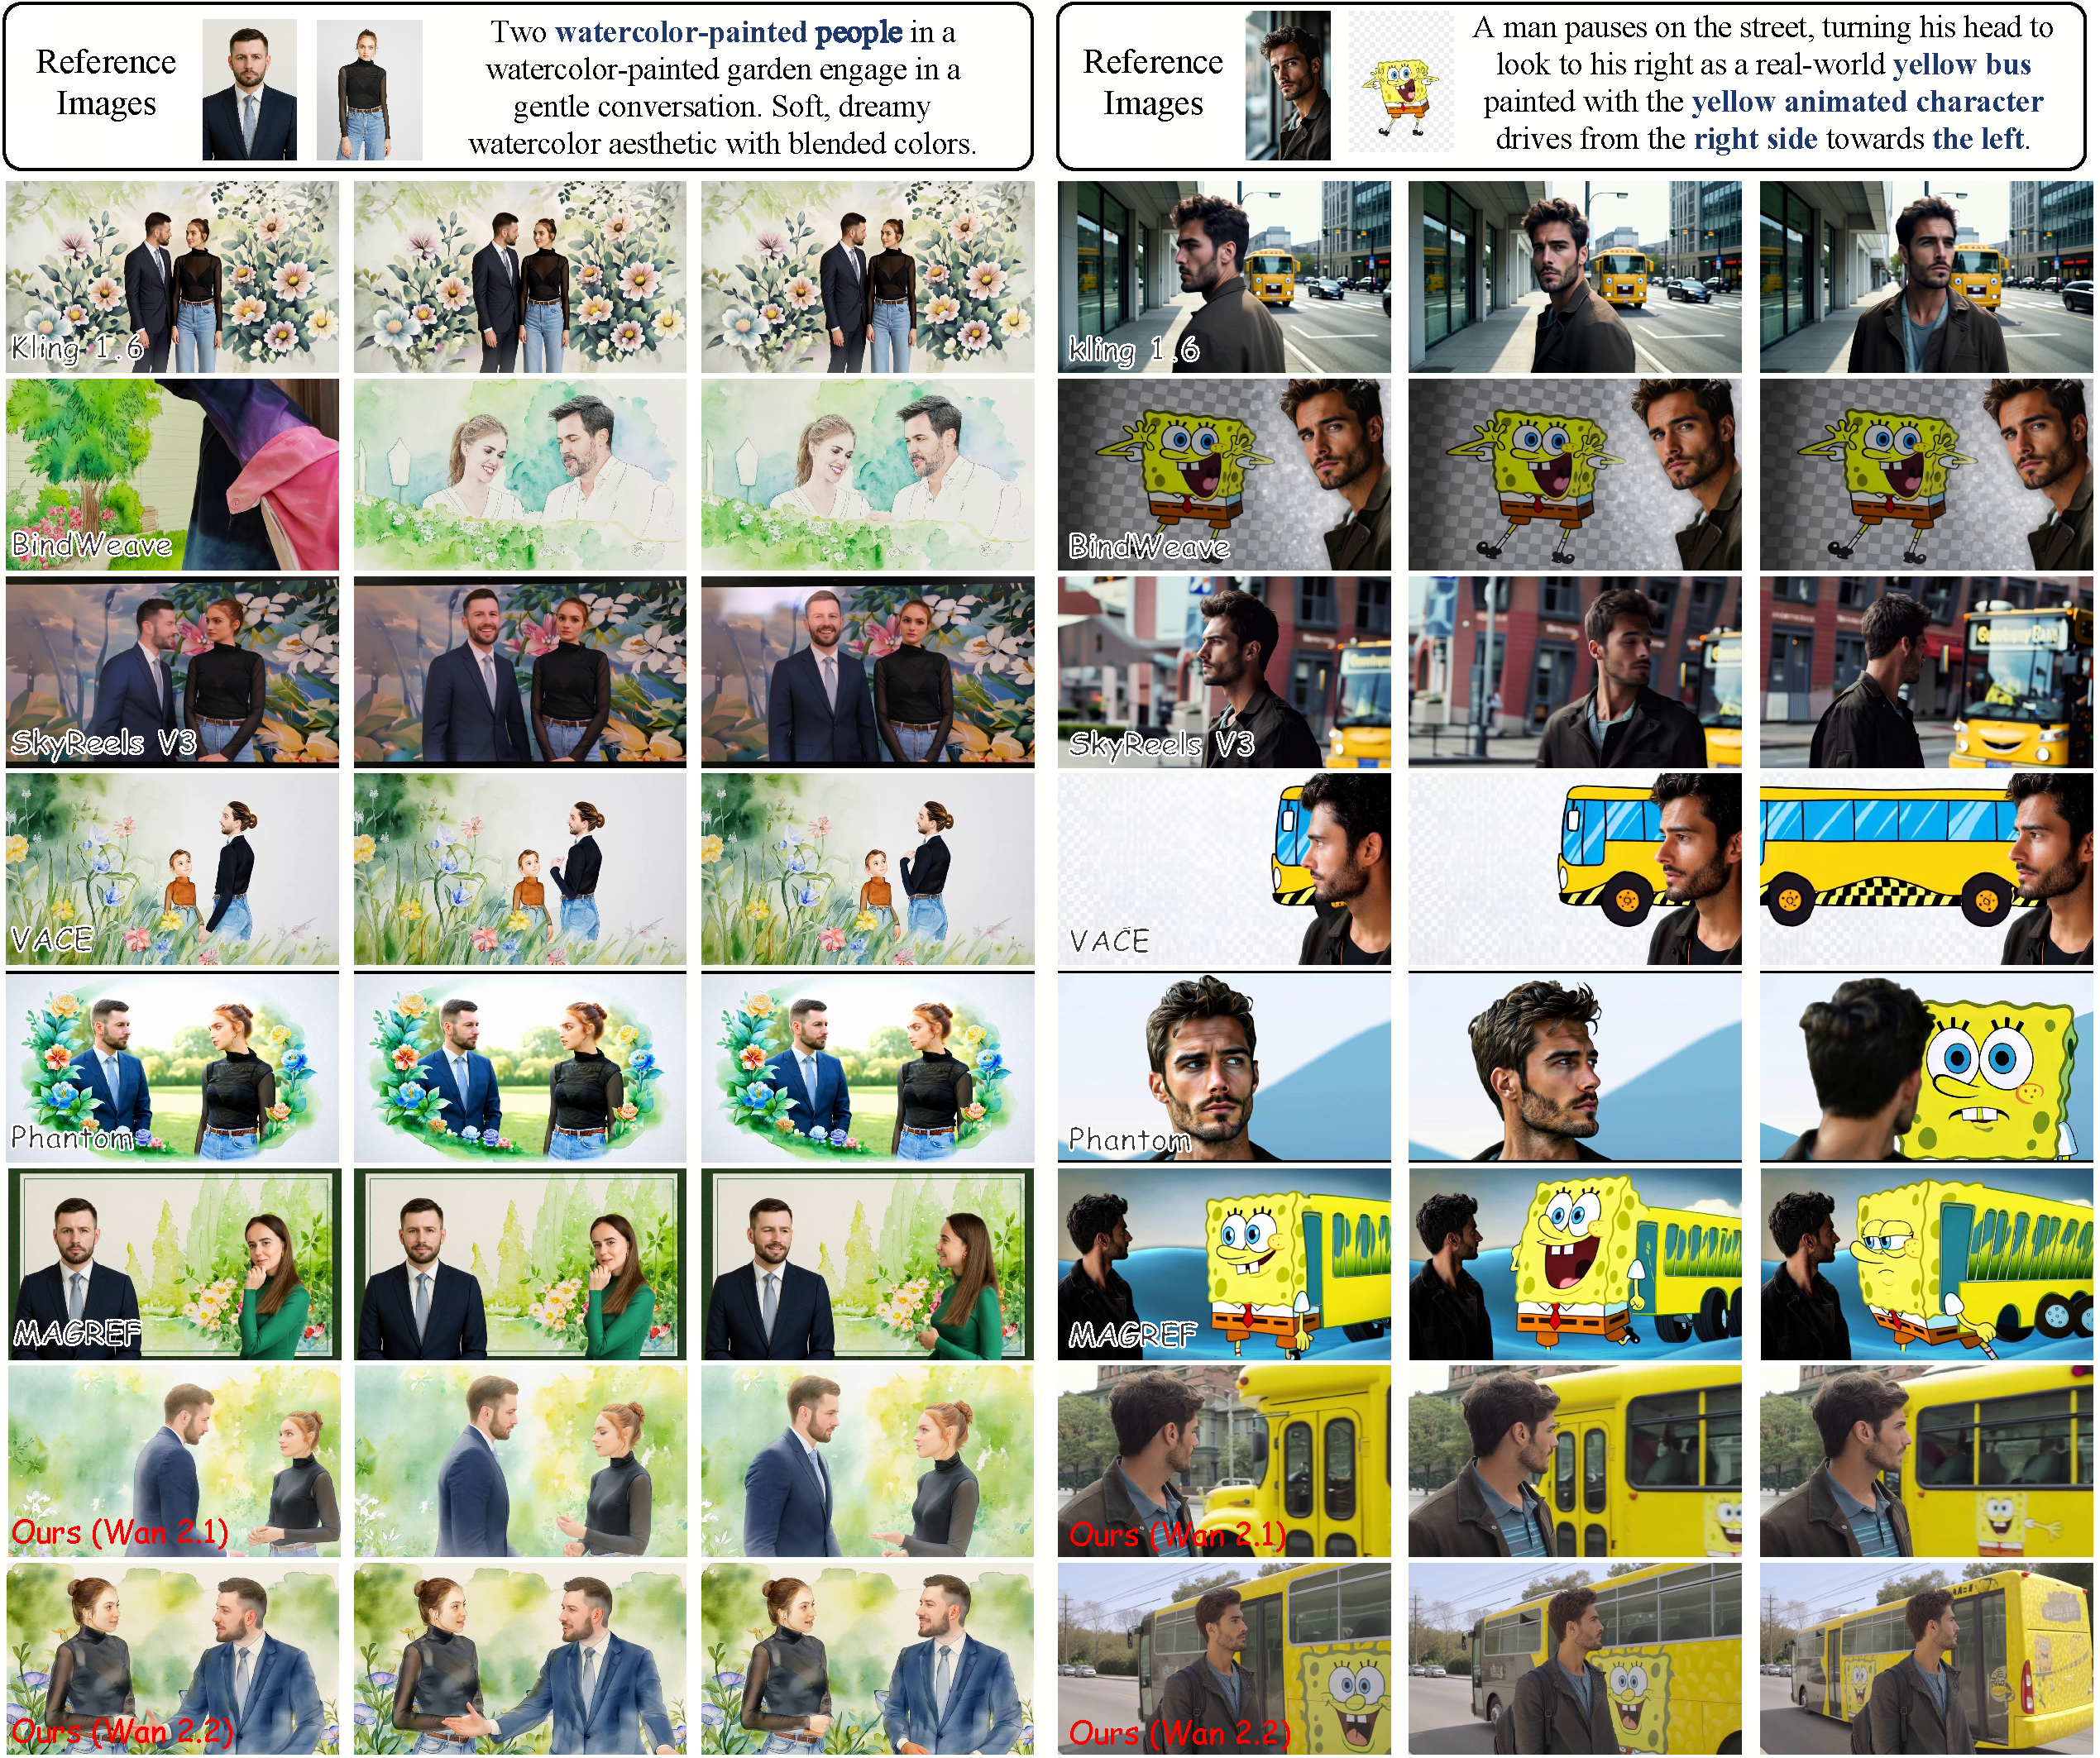
\includegraphics[width=0.98\linewidth]{figures/visual_case_1.pdf}
    \caption{\textbf{Qualitative comparison} with existing methods. \textit{DomainShuttle} outperforms existing methods in cross-domain scenarios, which achieves flexible text controllability (\eg, the yellow bus printed with the character) and precisely preserves the features of the reference subject. }
    \label{fig:visual_case}
\end{figure*}

\begin{figure*}[t]
    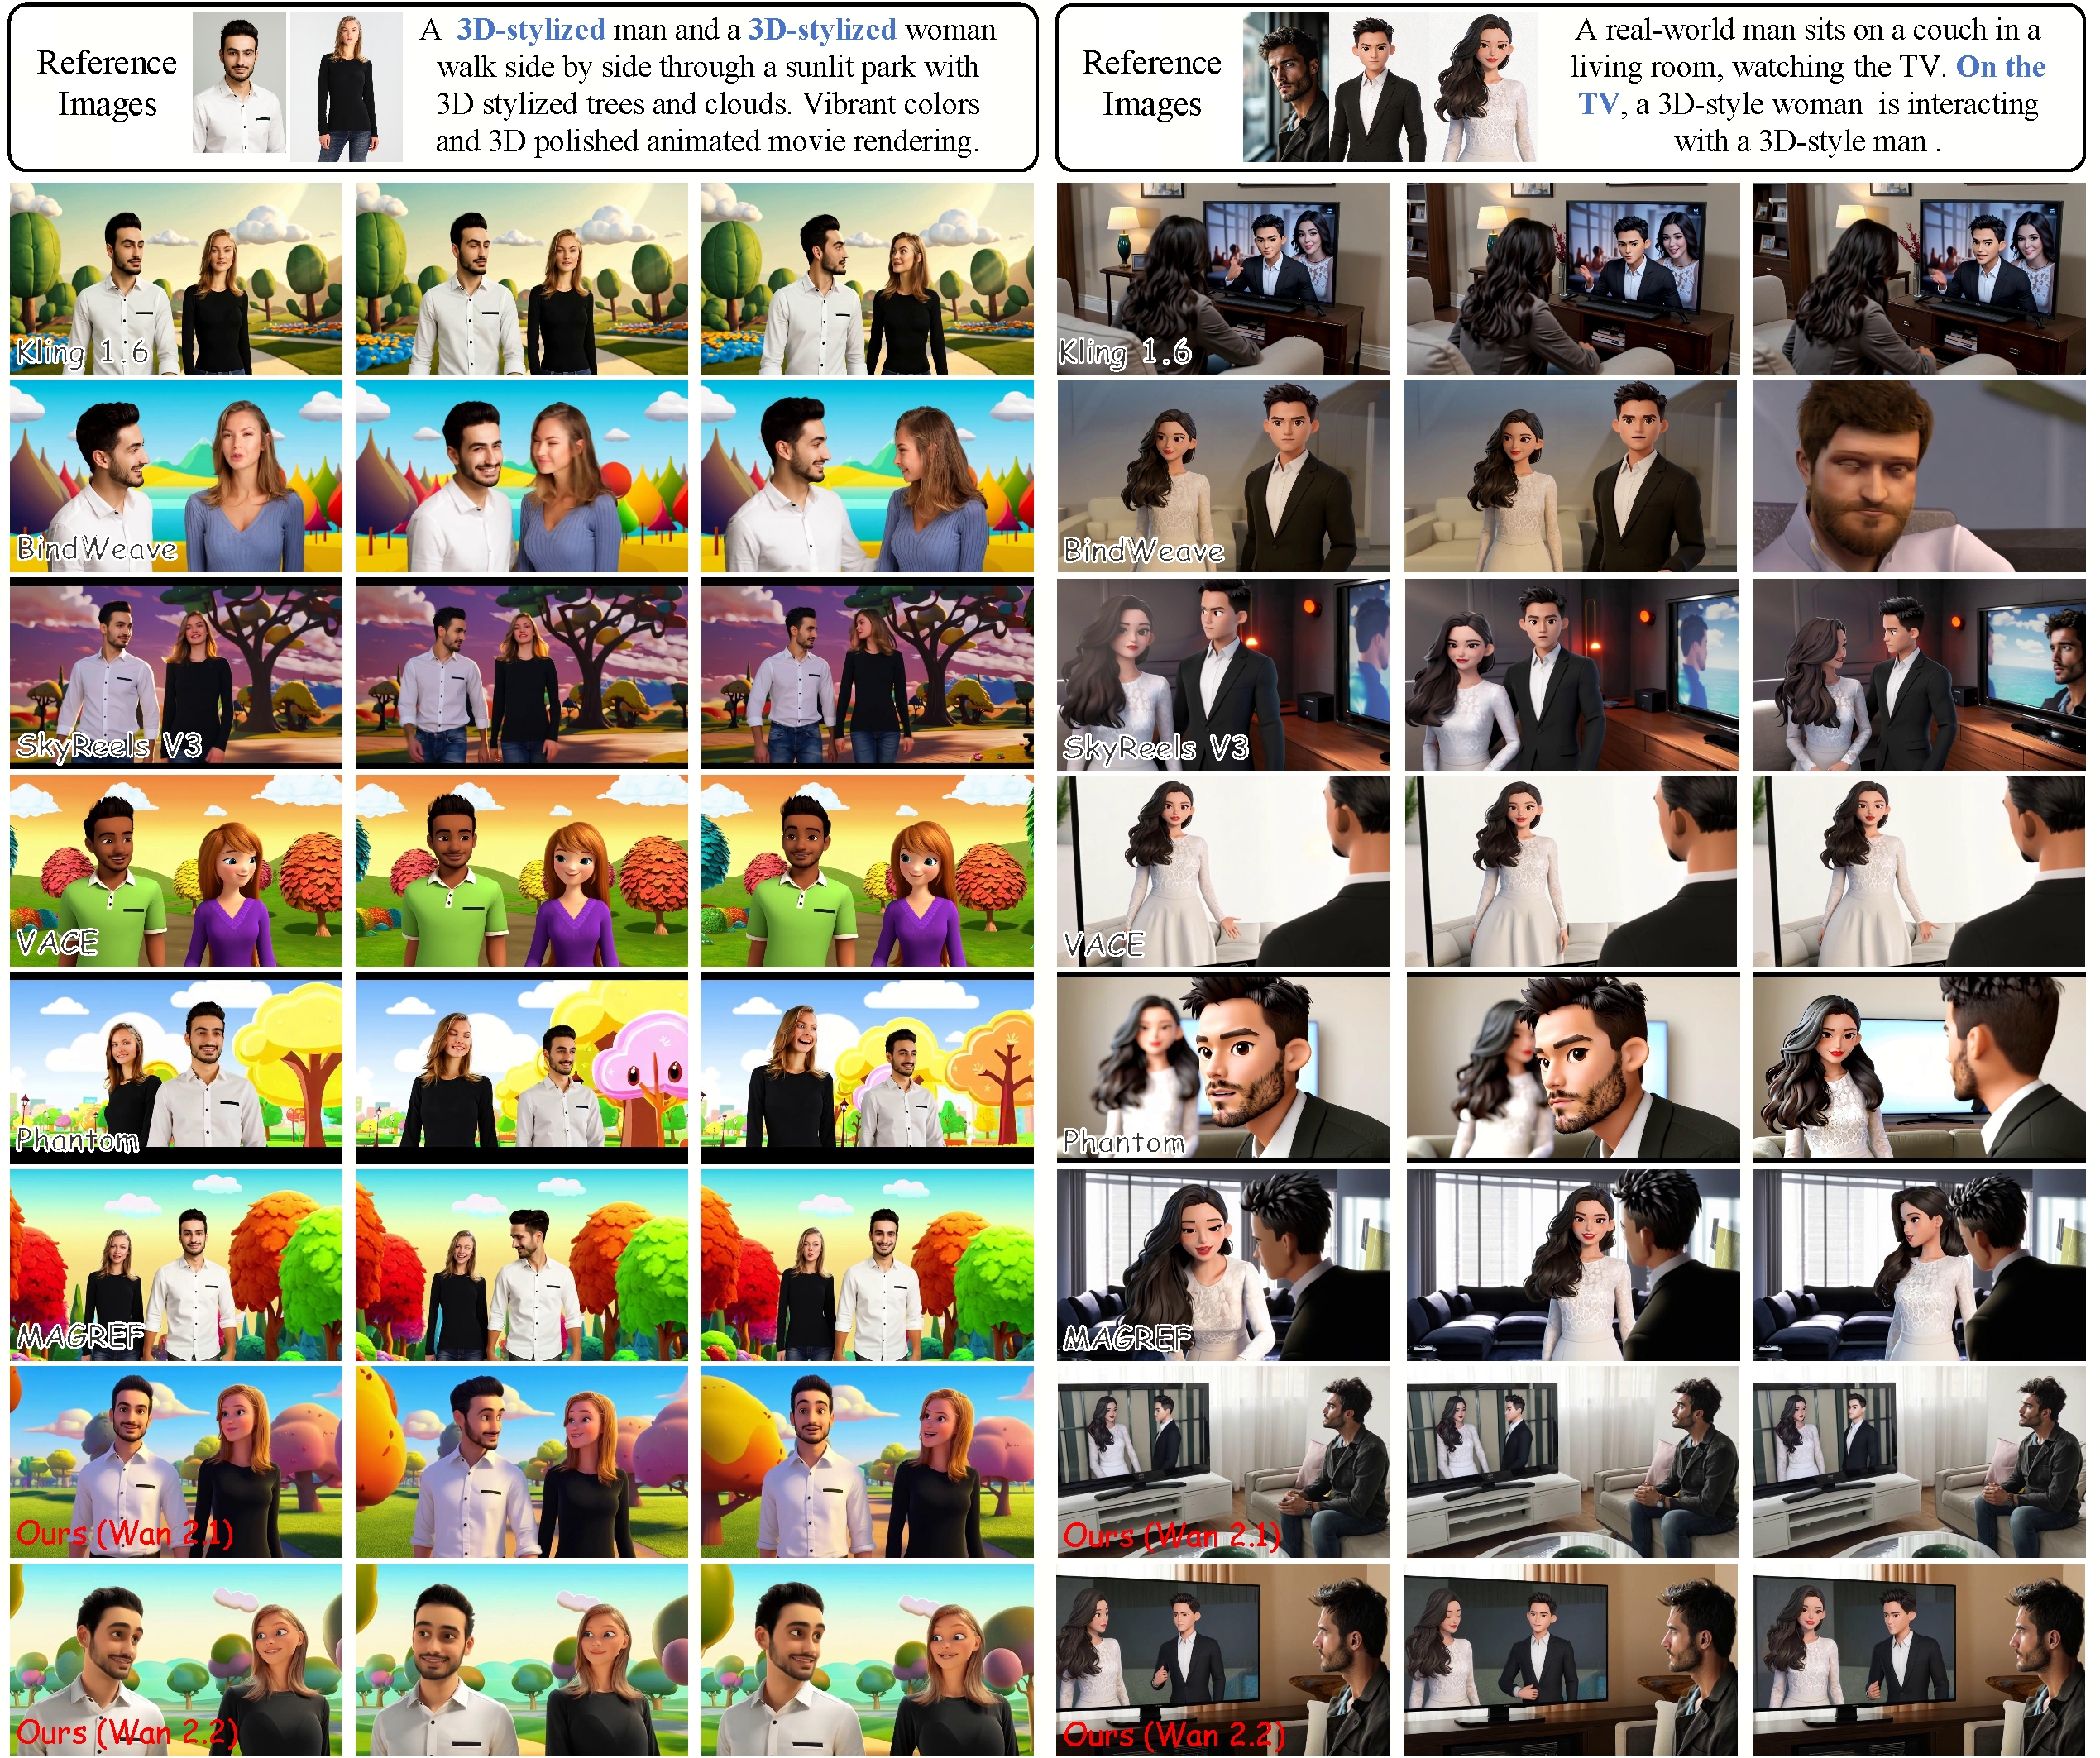
\includegraphics[width=0.98\linewidth]{figures/visual_case_2_changed.pdf}
    \caption{\textbf{More Qualitative comparison} with existing methods. \textit{DomainShuttle} further demonstrates strong performance in more challenging cross-domain scenarios. }
    \label{fig:visual_case_2}
\end{figure*}



\paragraph{\textbf{Evaluation Metrics.}} We evaluate the effectiveness of \textit{DomainShuttle} from three aspects. (1) Video Quality: The normalized Aesthetic Score (AES) and Motion Smoothness (MS) \cite{yuan2025opens2v} are used to evaluate the quality of videos generated by different methods. (2) Text Controllability: GMEScore\cite{gme} is used to evaluate text controllability. (3) Subject Consistency: We conduct evaluations under both In-Domain and Cross-Domain settings. For the In-Domain scenario, we adopt the standard DINO-I \cite{dinov2} and CLIP-I \cite{CLIP} metrics. Specifically, we first segment the subjects in videos and then compute subject-level similarity. 






For the \textbf{cross-domain} scenario, we design four metrics to evaluate different methods: NANO-CLIP, Qwen-CLIP, Cross-Domain (CD) Score, and Qwen-Score. NANO-CLIP and Qwen-CLIP use Nano-Banana Pro\cite{nano_banana} and Qwen-Image-Edit\cite{wu2025qwenimage}, respectively, to generate cross-domain reference images, and then compute the CLIP similarity between these reference images and the generated videos. CD-Score and Qwen-Score evaluate each method using GPT-5.2\cite{gpt52} and the open-source Qwen3-VL-8B-Instruct\cite{bai2025qwen3}, respectively. NANO-CLIP and Qwen-CLIP follow the same evaluation pipeline, differing only in the image editing model. Similarly, CD-Score and Qwen-Score differ only in the MLLM used. The use of an open-source MLLM improves the reproducibility of the metrics, while cross-model evaluation further enhances the reliability of the assessment. More evaluation details are shown in Sec. \ref{Experiments_Results} of the supplementary materials.


\paragraph{\textbf{Baselines.}} We conduct quantitative analysis with SOTA methods to evaluate the effectiveness of our model. These methods are divided into three categories: (1) closed-source model Kling1.6 \cite{kling}; (2) Wan2.1-14B-based models: VACE \cite{vace}, MAGREF \cite{deng2026magref}, SkyReels-V3 \cite{skyreelsv3}, Phantom \cite{phantom}, HuMo \cite{chen2025humo}, and BindWeave \cite{li2026bindweave}; (3) Wan2.2-14B-based models: FFGO \cite{chen2025first} and VACE-Wan2.2 \cite{vace}.
%

\subsection{Main results}
\paragraph{\textbf{Quantitative Results.}} The quantitative results are shown in Tab. \ref{tab:s2v_result}. Compared with baselines, \textit{DomainShuttle} achieves the best performance in motion smoothness and text controllability. Our method significantly outperforms baselines in most subject consistency metrics, particularly with a significant $18.7\%$  improvement in cross-domain (CD) score. These quantitative experiments demonstrate that \textit{DomainShuttle} can generate high-quality videos with competitive text controllability and subject consistency in open-domain scenarios.



\paragraph{\textbf{Qualitative Results.}} Fig. \ref{fig:visual_case} and Fig. \ref{fig:visual_case_2} illustrate the qualitative results compared to existing methods. Our method demonstrates high subject consistency and text controllability. For real-world subjects in fantasy domains, such as watercolor and 3D animation domains (Fig. \ref{fig:visual_case} and Fig. \ref{fig:visual_case_2}, left side), our method preserves the inherent subject features while successfully following the style instructions, whereas existing methods either fail to follow the style guidance or lose subject consistency while following the style guidance. Our method also successfully achieves mapping fantasy subjects to real-world objects (Fig. \ref{fig:visual_case}, right side), while the baseline either fails to attach the fantastic subject to the bus or only generates the fantastic subject. For interactions between real-world and fantastic subjects (Fig. \ref{fig:visual_case_2}, right side), \textit{DomainShuttle} also achieves the best performance, while other methods fail to generate correct subject interactions. %More qualitative results are detailed in the supplementary materials.



\subsection{Ablation Study}
To demonstrate the effectiveness of each essential module of \textit{DomainShuttle}, we conduct extensive ablation experiments. All ablation experiments are trained on the Wan2.2-14B-T2V with the same training steps.


\begin{table*}[t]
\centering
\caption{\textbf{Ablation Studies} of each essential module. }
\setlength\tabcolsep{10pt}
\resizebox{1.0\textwidth}{!}{%
\begin{tabular}{lcccccc}
\toprule
\multirow{2}{*}{ID} & \multirow{2}{*}{Setting} & Text Controllability  & \multicolumn{2}{c}{Cross-Domain Subject Consistency} & \multicolumn{2}{c}{In-Domain Subject Consistency} \\
 \cmidrule(lr){3-3} \cmidrule(lr){4-7} & &  GMEScore$\uparrow$ & NANO-CLIP$\uparrow$ & CD-Score$\uparrow$ & DINO-I $\uparrow$ & CLIP-I    $\uparrow$ \\

% ID & Setting & GMEScore $\uparrow$  & NANO-CLIP $\uparrow$ & GPT-Score $\uparrow$ & DINO-I $\uparrow$ & CLIP-I $\uparrow$ \\ 
\midrule
0 & Naive Method       & 0.664 & 0.601 & 0.697 & 0.356 & 0.675  \\
1 & 0 + Dual Self-Attn   & 0.671 & 0.609 & 0.715 & 0.367 & 0.683  \\
2 & 0 + Domain-MoT       & 0.687 & 0.627 & 0.783 & \underline{0.396} & \textbf{0.697}  \\
\midrule
3 & 2 + VR-DualRoPE& \underline{0.691} & \underline{0.629} & \underline{0.813} & 0.394 & 0.688  \\
4 & 3 +  CCL            & \textbf{0.705} & \textbf{0.636} & \textbf{0.861} & \textbf{0.400} & \underline{0.690}  \\  
\bottomrule
\end{tabular}%
}
\vspace{-4pt}
\label{tab:ablation}
\end{table*}

\begin{figure*}[t]
    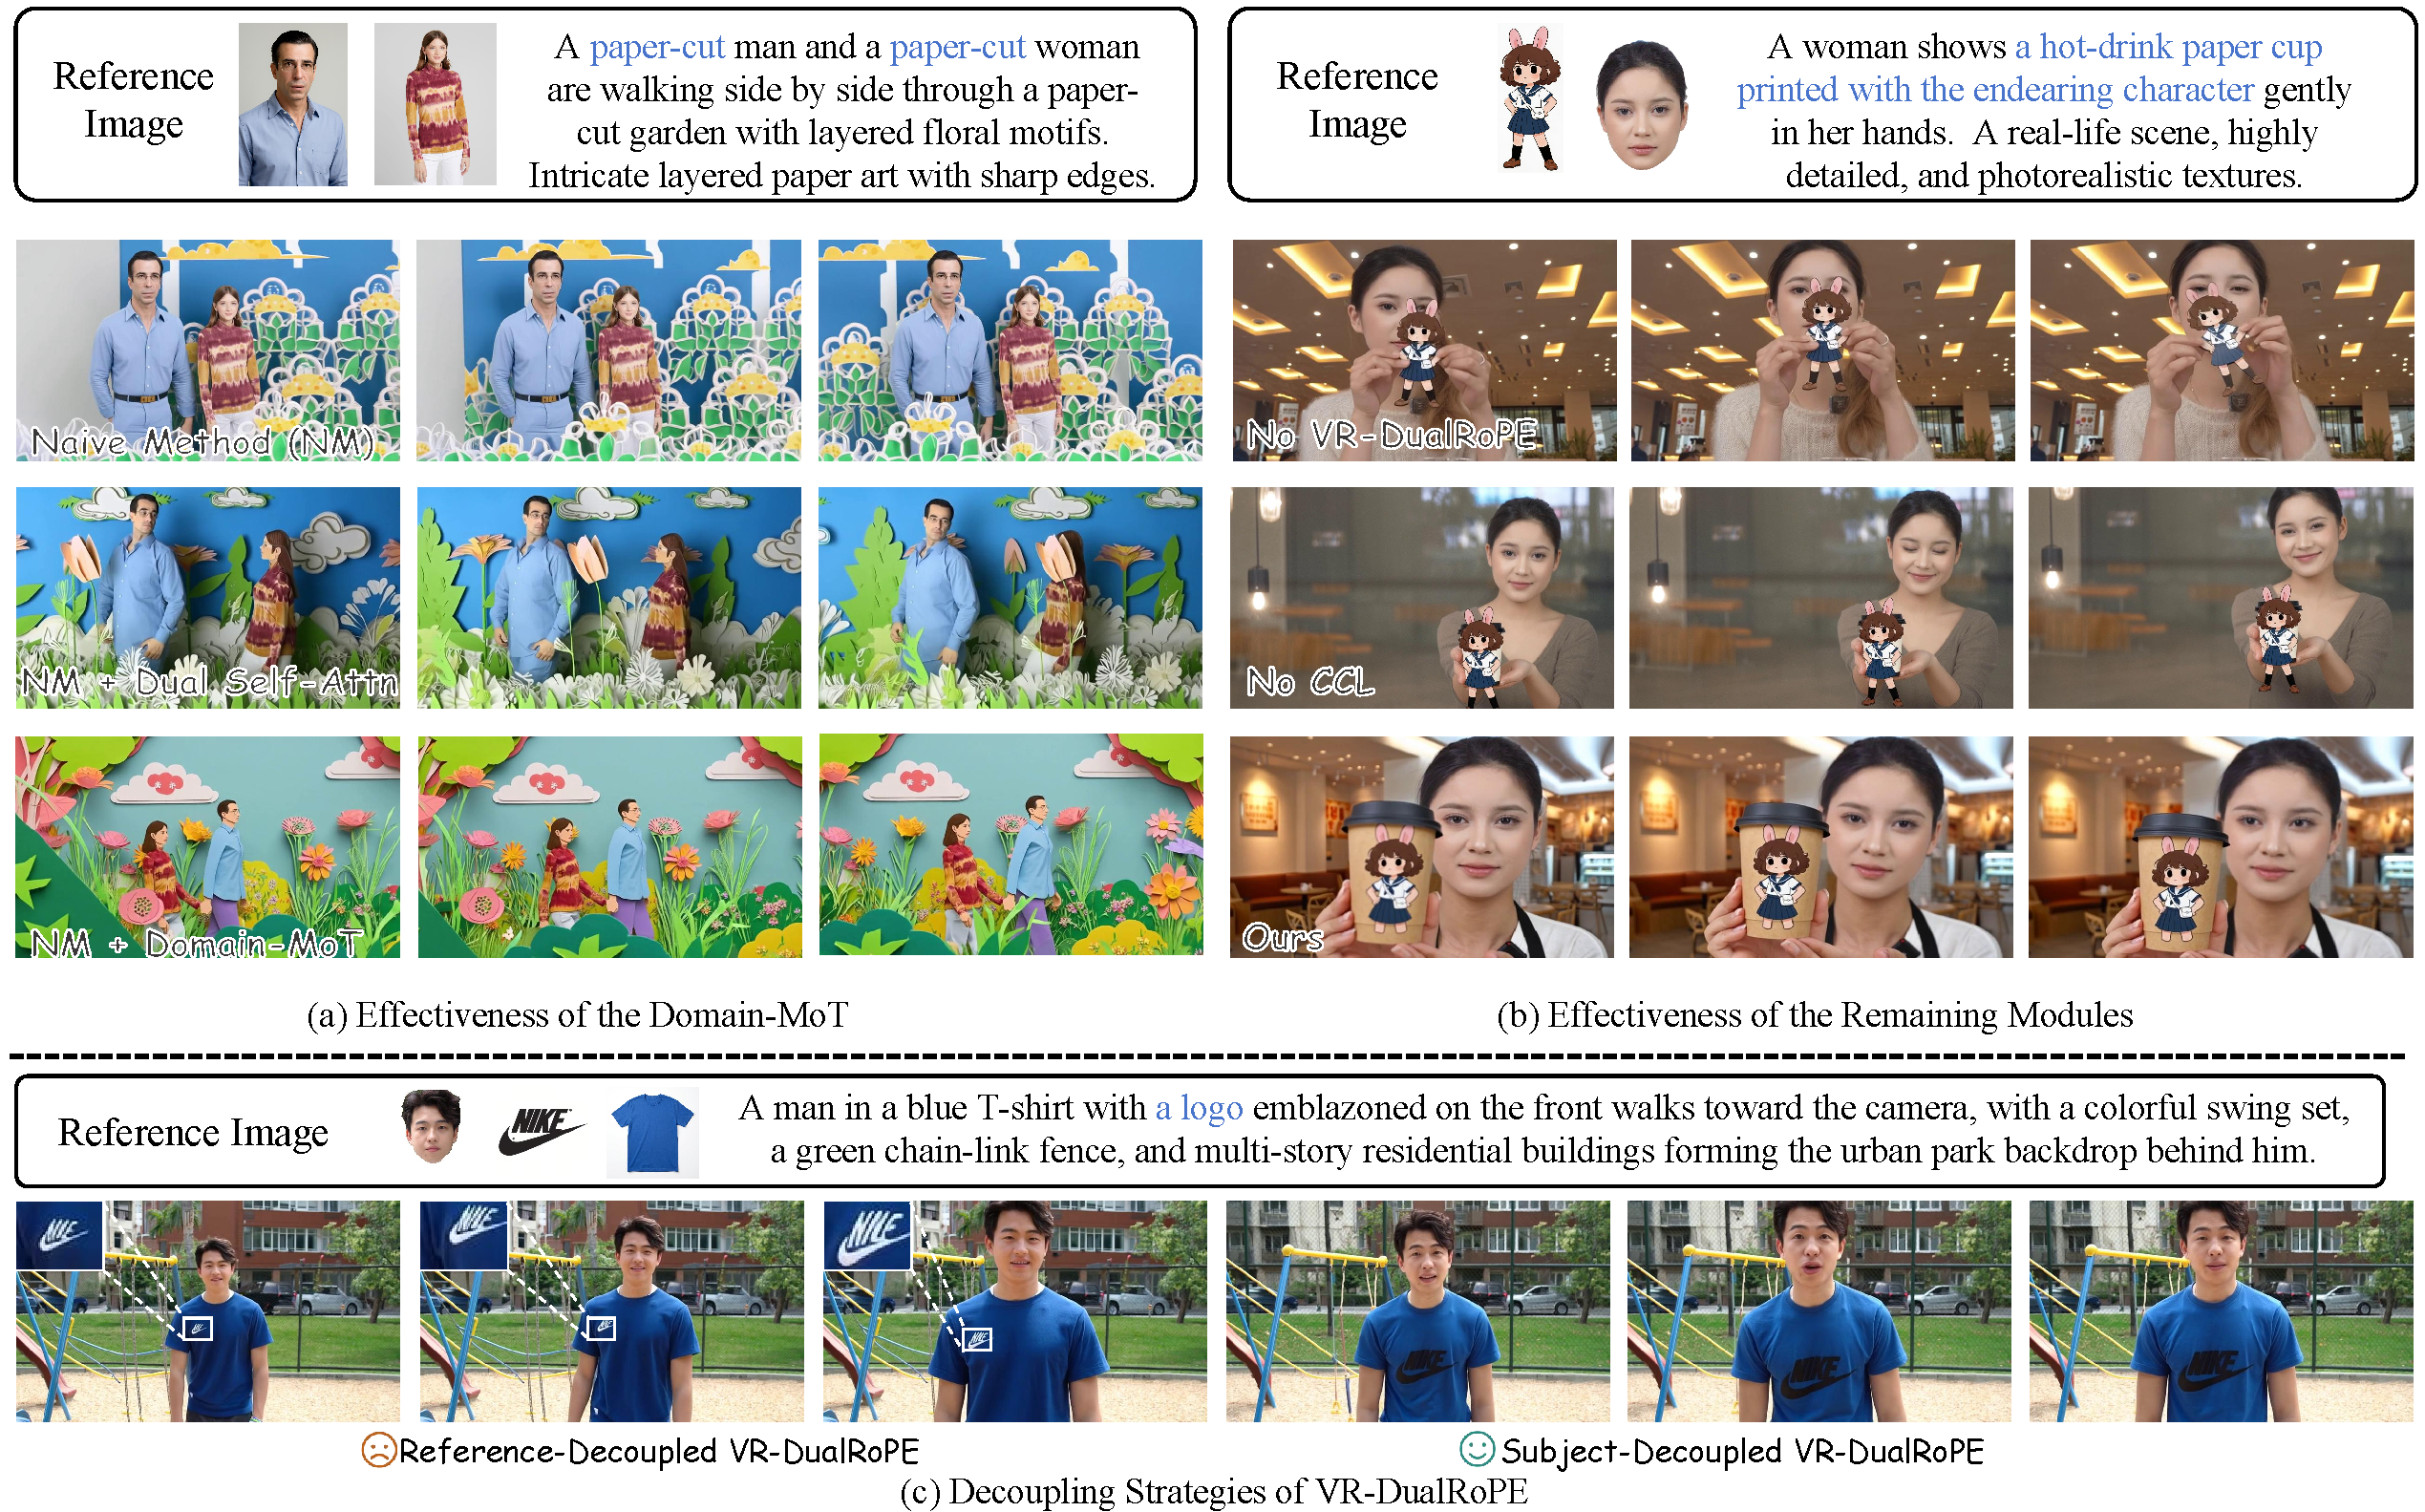
\includegraphics[width=0.98\linewidth]{figures/ablation_study_2.pdf}
    \caption{\textbf{Ablation Studies}. (a) Compared to Dual Self-Attn, Domain-MoT transfers all reference subjects into the fantasy domain. (b) Replacing VR-DualRoPE with naive RoPE causes incorrect subject interactions, while removing CCL induces direct copying from the reference. Using both yields the best results. (c) VR-DualRoPE uses a subject-decoupled offset to better bind these references than reference-decoupled offset.}
    \label{fig:ablation_fig}
\end{figure*}

\paragraph{\textbf{Effectiveness of the Domain-MoT.}}  Ablation results of Domain-MoT are shown in Tab. \ref{tab:ablation} and Fig. \ref{fig:ablation_fig} (a). The Naive Method refers to directly concatenating reference image tokens with video tokens without additional operations; Dual Self-Attn refers to introducing a dedicated attention mapping pathway for reference image tokens in self-attention. ID-0, ID-1, and ID-2 employ a naive RoPE scheme, in which the RoPE indices of the reference image tokens are concatenated to the video tokens along the temporal dimension. The Naive Method (ID-0) usually fails to transfer the reference subjects to the target fantasy domain. Dual Self-Attn (ID-1) partially improves domain transfer, but still cannot consistently transform all reference subjects. For instance, in  Fig. \ref{fig:ablation_fig} (a), only the woman is converted into the paper-cut style. In contrast, Domain-MoT (ID-2) successfully converts all humans into the target style. Quantitatively, Domain-MoT improves the CD-Score from 0.697 to 0.783 compared to the Naive Method.






\paragraph{\textbf{Effectiveness of the Remaining Modules.}} The ablation results of Video-Reference (VR) DualRoPE and CCL are shown in Tab. \ref{tab:ablation} and Fig. \ref{fig:ablation_fig} (b). Replacing VR-DualRoPE with the naive RoPE scheme causes the reference image to be treated as a video frame in the RoPE space, leading to incorrect subject interactions and weaker editability. Without VR-DualRoPE, the animated character appears at an incorrect spatial position and fails to attach to the paper cup held by the person, as shown in Fig. \ref{fig:ablation_fig} (b). Removing CCL causes the model to directly copy the object from the reference image, indicating that CCL facilitates learning more precise representations of the reference subject. CCL mainly improves \textbf{controllability} in cross-domain scenarios, rather than fidelity. As shown in Tab. \ref{tab:ablation} of the main submission, CCL improves fidelity by only 0.3\% (CLIP) and 1.5\% (DINO), but significantly improves CD-Score by \textbf{5.9\%}, supporting this point. Combining VR-DualRoPE and CCL, \textit{DomainShuttle} (ID-4) achieves the best performance.




%update here

\paragraph{\textbf{Decoupling Strategies of VR-DualRoPE.}} In some open-domain scenarios, multiple reference images may represent different attributes of the same subject. To address this, Video-Reference DualRoPE adopts a strategy in which multiple reference images of the same subject are offset only along the width dimension in RoPE, rather than applying offsets along both height and width for different reference images by default. As shown in Fig. \ref{fig:ablation_fig} (c), compared with the reference-decoupled strategy, the subject-decoupled strategy better binds multiple reference images of the same subject.


\subsection{Human Preference Evaluation}



We invite $40$ volunteers to conduct a human preference evaluation comparing \textit{DomainShuttle} with well-performed methods. Each person ranks $20$ randomly selected videos in three aspects: video quality, text controllability, and open-domain subject consistency. Distinct scores from 5 (best) to 1 (worst) are assigned to different methods without ties. As shown in Fig. \ref{fig:user_study}, our method achieves superior performance in all metrics, showing significant advantages in open-domain subject consistency, validating the effectiveness of \textit{DomainShuttle}.



\begin{figure*}[t]
    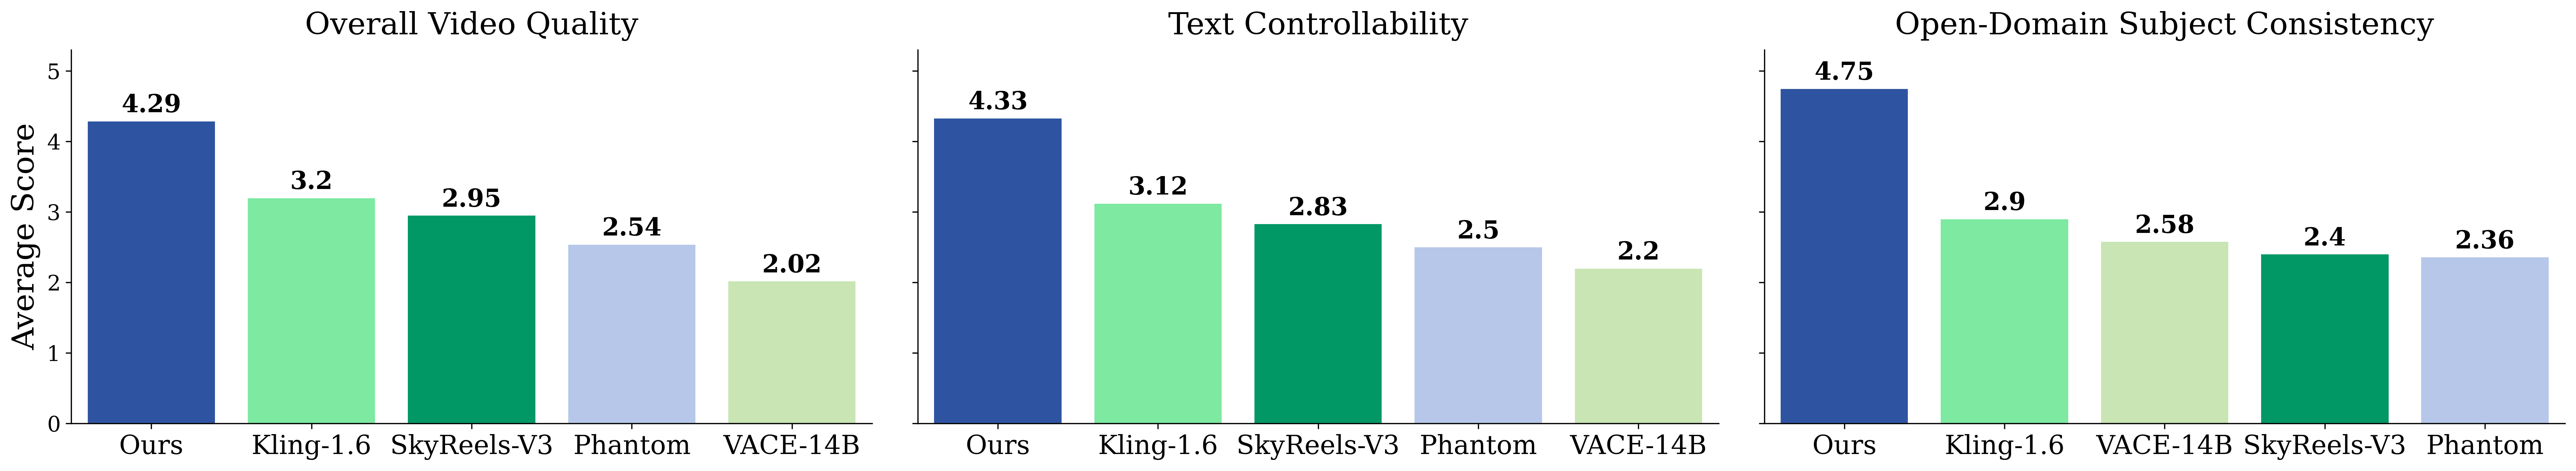
\includegraphics[width=0.98\linewidth]{figures/user_study_2.png}
    \caption{\textbf{Human preference evaluation}. \textit{DomainShuttle} significantly outperforms baselines in video quality, text controllability, and open-domain subject consistency.}
    \label{fig:user_study}
\end{figure*}
